\section{Supplementary Results}
\label{sec:appendix}

%-------------------------------------------------------------------
\subsection{Encoder Ablation}
\label{sec:app_encoder}

\begin{table}[h]
\centering
\small
\begin{tabular}{lccccc}
\toprule
\textbf{Encoder} & \textbf{Dim} & \textbf{Macro-F1} & \textbf{F1\textsubscript{stag}} & \textbf{F1\textsubscript{prog}} & \textbf{Best Ep.} \\
\midrule
Qwen3-0.6B & 1024 & 0.9055 & --- & --- & --- \\
E5-large-v2 & 1024 & $0.9405 \pm 0.0030$ & --- & --- & --- \\
BGE-M3 & 1024 & \textbf{0.9413} & \textbf{0.9147} & \textbf{0.9679} & 5 \\
\bottomrule
\end{tabular}
\caption{Encoder ablation on SWE-Agent conf${\geq}$2 ($N{=}1{,}824$). All models use the same GRU architecture (2-layer, hidden$=$256, dropout$=$0.1, lr$=$1e-3, batch$=$32, early stopping patience~5). All encoders exceed 0.90 macro-F1, confirming the probe's temporal architecture drives performance rather than a specific encoder. BGE-M3 achieves the highest score ($+$3.6\,pp over Qwen3), but the gap between encoders (0.5\,pp) is small relative to the structural--probe gap (8.96\,pp). ``---'' indicates per-class scores were not logged in the initial sweep; macro-F1 is computed from the checkpoint with lowest validation loss. E5-large-v2 reports mean $\pm$ std over 3 seeds.}
\label{tab:encoder_ablation}
\end{table}

%-------------------------------------------------------------------
\subsection{Window Size Ablation}
\label{sec:app_window}

\begin{table}[h]
\centering
\small
\begin{tabular}{ccccc}
\toprule
\textbf{Window $k$} & \textbf{Macro-F1} & \textbf{F1\textsubscript{stag}} & \textbf{F1\textsubscript{prog}} & \textbf{$\Delta$ vs.\ $k{=}5$} \\
\midrule
3 & 0.8721 & 0.7784 & 0.9659 & $-$5.9\,pp \\
\textbf{5} & \textbf{0.9309} & \textbf{0.8917} & \textbf{0.9701} & --- \\
7 & 0.9133 & 0.8791 & 0.9475 & $-$1.8\,pp \\
\bottomrule
\end{tabular}
\caption{Window size ablation on SWE-Agent conf${\geq}$2 using the Qwen3-0.6B encoder (seed~42). $k{=}5$ is optimal. $k{=}3$ lacks sufficient context for stagnation detection (F1\textsubscript{stag} drops 11.3\,pp). $k{=}7$ dilutes signal by spanning both progress and stagnation phases.}
\label{tab:window_ablation}
\end{table}

%-------------------------------------------------------------------
\subsection{Multi-Seed Stability}
\label{sec:app_multiseed}

\begin{table}[h]
\centering
\small
\begin{tabular}{lcccc}
\toprule
\textbf{Method} & \textbf{In-Domain F1} & \textbf{Seeds} & \textbf{Cross-Agent F1} & \textbf{Seeds} \\
\midrule
Structural RF & $0.9951 \pm 0.0000$ & 5 & --- & --- \\
Structural GB & --- & --- & $0.9678 \pm 0.0015$ & 5 \\
ProgressProbe (GRU) & $0.9185 \pm 0.0113$ & 5 & --- & --- \\
\bottomrule
\end{tabular}
\caption{Multi-seed stability (mean $\pm$ std). In-domain: SWE-Agent conf${\geq}$2; cross-coding-agent: SWE-Agent $\to$ OpenHands zero-shot transfer. Structural classifiers show zero or near-zero variance. The probe exhibits higher variance ($\sigma{=}0.011$) but all seeds exceed 0.90. ``---'' indicates the setting was not evaluated: RF is evaluated in-domain only, GB cross-coding-agent only, and the probe in-domain only.}
\label{tab:multiseed}
\end{table}

%-------------------------------------------------------------------
\subsection{Cross-Agent Label Quality and Few-Shot Transfer}
\label{sec:app_cmdrep}

Table~\ref{tab:cross_agent_cmdrep} extends the label quality analysis from \S\ref{sec:cmd_rep_ablation}, showing probe fine-tuning performance across data fractions under corrected OH labels.

\begin{table}[h]
\centering
\small
\begin{tabular}{lc}
\toprule
\textbf{OH Data Fraction} & \textbf{Probe Macro-F1} \\
\midrule
0\% (zero-shot) & 0.598 \\
5\% & 0.850 \\
10\% & 0.918 \\
20\% & 0.948 \\
50\% & 0.968 \\
100\% & 0.976 \\
\bottomrule
\end{tabular}
\caption{Probe fine-tuning on corrected OH labels across data fractions. The zero-shot--to--5\% jump ($+$25.2\,pp) and rapid convergence toward structural GB (0.992 on conf${\geq}$2) demonstrate that label quality, not model capacity, was the transfer bottleneck. Under old (corrupted) labels, 5\% fine-tuning reached only 0.570.}
\label{tab:cross_agent_cmdrep}
\end{table}

The probe reaches 0.948 macro-F1 at 20\% OH data---within 5\,pp of structural GB on conf${\geq}$2 windows (0.992)---and at 50\% (0.968) closes to within 2.5\,pp of structural GB on conf${\geq}$2 (0.992).
This rapid convergence under corrected labels contrasts sharply with the old label regime, where even 100\% fine-tuning reached only 0.751.
The improvement is driven entirely by label quality: the model architecture and training procedure are identical.

Under the prevalence-matched ablation (\S\ref{sec:cmd_rep_ablation}), 3-LF and 2-LF label sets agree on 100\% of overlapping windows, confirming that cmd\_rep's contribution is coverage (expanding conf${\geq}$2 training data from ${\sim}$4K to ${\sim}$43K windows) rather than label refinement.
The $-29.4$\,pp drop upon removing cmd\_rep (McNemar $\chi^2{=}1{,}551$, $p{\approx}0$) is thus attributable to data volume collapse, not label noise.

%-------------------------------------------------------------------
\subsection{Structural Feature Definitions}
\label{sec:app_features}

Table~\ref{tab:feature_defs} lists all 30 structural features with their categories and LF overlap classification.
A feature is classified as LF-overlapping if it is computed from the same signal space that any labeling function uses as input (\S\ref{sec:feature_overlap}).

\begin{table*}[h]
\centering
\small
\begin{tabular}{rlll}
\toprule
\textbf{\#} & \textbf{Feature} & \textbf{Category} & \textbf{LF Overlap} \\
\midrule
1  & num\_steps             & Trajectory stats    & --- \\
2  & num\_actions           & Trajectory stats    & --- \\
3  & num\_observations      & Trajectory stats    & --- \\
4  & action\_ratio          & Trajectory stats    & --- \\
5  & mean\_text\_len        & Text statistics     & --- \\
6  & std\_text\_len         & Text statistics     & --- \\
7  & max\_text\_len         & Text statistics     & --- \\
8  & min\_text\_len         & Text statistics     & --- \\
9  & mean\_action\_len      & Text statistics     & --- \\
10 & mean\_obs\_len         & Text statistics     & --- \\
11 & text\_len\_trend       & Text statistics     & --- \\
12 & num\_commands          & Command stats       & --- \\
13 & mean\_cmd\_len         & Command stats       & --- \\
14 & max\_cmd\_len          & Command stats       & --- \\
15 & unique\_cmd\_ratio     & Repetition          & $\lambda_1$ \\
16 & max\_repeat\_ratio     & Repetition          & $\lambda_1$ \\
17 & num\_edit\_cmds        & File operations     & $\lambda_2$ \\
18 & num\_search\_cmds      & File operations     & $\lambda_2$ \\
19 & num\_nav\_cmds         & File operations     & --- \\
20 & num\_submit\_cmds      & File operations     & --- \\
21 & edit\_ratio            & File operations     & $\lambda_2$ \\
22 & search\_ratio          & File operations     & $\lambda_2$ \\
23 & avg\_adjacent\_cmd\_sim & Edit distance       & $\lambda_1$ \\
24 & max\_adjacent\_cmd\_sim & Edit distance       & $\lambda_1$ \\
25 & max\_consec\_similar   & Edit distance       & $\lambda_1$ \\
26 & num\_errors            & Output statistics   & --- \\
27 & num\_test\_outputs     & Output statistics   & --- \\
28 & num\_file\_displays    & Output statistics   & $\lambda_2$ \\
29 & num\_nonzero\_exits    & Output statistics   & --- \\
30 & is\_short\_trajectory  & Trajectory stats    & $\lambda_3$ \\
\bottomrule
\end{tabular}
\caption{Complete structural feature definitions ($N{=}30$). LF Overlap indicates which labeling function's signal space the feature shares: $\lambda_1$ (command repetition), $\lambda_2$ (file diff), $\lambda_3$ (outcome backpropagation), or ``---'' (no overlap). 11 features overlap with at least one LF; 19 are residual.}
\label{tab:feature_defs}
\end{table*}

%-------------------------------------------------------------------
\subsection{Instance Isolation}
\label{sec:app_instance_isolation}

\begin{table}[h]
\centering
\small
\begin{tabular}{lccc}
\toprule
\textbf{Model} & \textbf{Full} & \textbf{Unseen-only} & \textbf{$\Delta$} \\
\midrule
GB all & 0.9674 & 0.9669 & $-$0.05\,pp \\
RF all & 0.9123 & 0.9121 & $-$0.01\,pp \\
GB conf${\geq}$2 & 0.9919 & 0.9917 & $-$0.02\,pp \\
RF conf${\geq}$2 & 0.9959 & 0.9962 & $+$0.03\,pp \\
\bottomrule
\end{tabular}
\caption{Instance isolation: cross-coding-agent macro-F1 with and without 284 SWE-bench task instances that overlap between the 1,386 SWE-bench training instances and 3,409 OH test instances (8.3\% of OH). All $|\Delta| < 0.1$\,pp, confirming transfer reflects behavioral pattern generalization rather than instance memorization.}
\label{tab:instance_isolation}
\end{table}

%-------------------------------------------------------------------
\subsection{Extended LLM-as-Judge Evaluation}
\label{sec:llm_extended}

Table~\ref{tab:llm_extended} extends the zero-shot LLM-as-judge baseline (Table~\ref{tab:main_results}) with chain-of-thought (CoT) prompting, few-shot examples, and an alternative model, all evaluated on the SWE-Agent conf${\geq}$2 test set ($N{=}1{,}824$).

\begin{table}[h]
\centering
\small
\begin{tabular}{llcccc}
\toprule
\textbf{Model} & \textbf{Setting} & \textbf{Macro-F1} & \textbf{F1\textsubscript{stag}} & \textbf{F1\textsubscript{prog}} & \textbf{Cost} \\
\midrule
Claude Sonnet 4.6 & zero-shot & 0.6625 & 0.6055 & 0.7195 & \$11.66 \\
Claude Sonnet 4.6 & CoT & 0.7499 & 0.6808 & 0.8189 & \$17.16 \\
Claude Sonnet 4.6 & 5-shot & 0.7514 & 0.6828 & 0.8199 & \$36.08 \\
Claude Sonnet 4.6 & 5-shot-CoT & \textbf{0.7994} & \textbf{0.7306} & \textbf{0.8681} & \$40.56 \\
GPT-5.5$^\dagger$ & zero-shot & 0.7465 & 0.7110 & 0.7819 & \$11.62 \\
\midrule
\multicolumn{6}{l}{\emph{Structural feature augmentation}} \\
Claude Sonnet 4.6 & + structural input$^\ddagger$ & 0.6880 & 0.6270 & 0.7490 & \$14.82 \\
\bottomrule
\end{tabular}
\caption{Extended LLM-as-judge evaluation on SWE-Agent conf${\geq}$2 ($N{=}1{,}824$). All Claude rows use the same model; the performance gain comes from prompting strategy. CoT alone yields gains comparable to few-shot ($+$8.7\,pp vs.\ $+$8.9\,pp over zero-shot); combining them (five-shot-CoT) adds a further 4.8\,pp, suggesting complementary mechanisms. $^\ddagger$30 structural features provided as formatted text in the LLM prompt; performance degrades below pure few-shot (0.7514), indicating structural signals require engineered classifiers. $^\dagger$GPT-5.5: 22.4\% of responses (408/1,824) failed to parse; macro-F1 is computed over the 1,416 windows with valid outputs. On silver, the best LLM (0.799) trails structural features (0.995); on gold, the ranking reverses (LLM 0.910 vs.\ GB 0.839; \S\ref{sec:gold_set}). Total API cost across all configurations: \$131.90.}
\label{tab:llm_extended}
\end{table}

%-------------------------------------------------------------------
\subsection{Temporal Label Model Specifications}
\label{sec:app_temporal_models}

\subsubsection{Time-Varying Weights (TWV)}

TWV applies Gaussian kernel smoothing to each LF's activation sequence:
\begin{equation}
\tilde{\lambda}_j(t) = \sum_{t'} K_\sigma(t - t') \cdot \lambda_j(t')
\label{eq:twv}
\end{equation}
where $K_\sigma$ is a Gaussian kernel with bandwidth $\sigma$.
Smoothed activations replace raw votes for conf${=}1$ windows (where exactly one LF disagrees), potentially flipping labels in temporally ambiguous regions.
The bandwidth $\sigma$ controls the extent of temporal context: larger values incorporate more distant steps.

\subsubsection{Hidden Markov Models}

We model the label sequence as a Hidden Markov Model \citep{safranchik2020linkedhmm} with two hidden states (stagnation, progress) and observations defined by the joint activation pattern of the three LFs.
Transition and emission parameters are estimated via Expectation-Maximization (EM).
The HMM captures temporal persistence---stagnation episodes tend to span multiple consecutive windows---which majority vote, operating independently per window, cannot model.

\subsubsection{Lag-Aware HMM}

The standard HMM treats all LFs as synchronous.
Lag-Aware HMM extends this by explicitly modeling each LF's temporal offset: $\lambda_1$ is shifted by $-2$ steps, $\lambda_2$ by $-1$, and $\lambda_3$ by $+7$, estimated from the temporal dynamics analysis (\S\ref{sec:lf_temporal}).
To prevent divergence, we apply two regularization strategies: (1)~\emph{confidence anchoring}, which fixes labels for conf${\geq}$2 windows and restricts EM updates to conf${=}1$ windows; and (2)~a prior strength of 5000 on transition parameters.
These constraints keep the model close to the majority vote baseline while allowing it to resolve temporally ambiguous labels.

%-------------------------------------------------------------------
\subsection{Label Quality: Extended Analysis}
\label{sec:app_label_quality}

With corrected labels, the 3-LF probe improves from zero-shot 0.598 to fine-tuned 0.976 (previously 0.7512 under corrupted labels).
The improvement is most dramatic at low data fractions: 5\% fine-tuning reaches 0.850, exceeding the old 50\% result (0.69) by 16.0\,pp.
The probe converges rapidly: at 50\% OH data it reaches 0.968, essentially matching structural GB (0.967).

The 29.4\,pp drop upon removing cmd\_rep is not caused by label accuracy improvement.
After correction, cmd\_rep fires on only 5.39\% of OH windows (down from the previously reported 92.2\% under corrupted embeddings) with 97.91\% precision---a high-precision, low-recall signal.
On the 4,070 windows where both 2-LF and 3-LF labels are defined, the two configurations agree on 100\% of labels: cmd\_rep does not change any label where the other two LFs already vote.
Its contribution is purely \emph{coverage}: including cmd\_rep expands the training set from ${\sim}$4K to ${\sim}$43K windows (a ${\sim}$10$\times$ increase).
The 2-LF model's low F1 reflects data volume collapse---too few training examples to learn the stagnation distribution---rather than label corruption.

These results reframe how labeling functions contribute to weak supervision pipelines.
A high-precision, low-recall LF like cmd\_rep may appear redundant when its labels are a subset of the majority vote, yet removing it causes training data to collapse by an order of magnitude.
The core contribution of such LFs is coverage provision, not label refinement.

%-------------------------------------------------------------------
\subsection{Temporal Label Model Results}
\label{sec:app_tlm_results}

\begin{table}[h]
\centering
\small
\begin{tabular}{lcccc}
\toprule
\textbf{Method} & \textbf{MV Agr.} & \textbf{Conf${\geq}$2 F1} & \textbf{$\Delta$ vs MV} & \textbf{Probe F1$^\ddagger$} \\
\midrule
MV (baseline) & 1.000 & 0.8946$^\ast$ & --- & 0.8468 \\
\midrule
\multicolumn{5}{l}{\emph{Temporal}} \\
TWV ($\sigma{=}2$) & 0.885 & \textbf{0.9003} & $+$0.6\,pp & 0.8211 \\
Lag-HMM & 0.820 & 0.8936 & $-$0.1\,pp & --- \\
HMM & 0.685 & 0.7502 & $-$14.4\,pp & 0.6564 \\
\midrule
\multicolumn{5}{l}{\emph{Generative (i.i.d.)}} \\
FlyingSquid & 0.820 & 0.7820 & $-$11.3\,pp & --- \\
Snorkel MeTaL & 0.423 & 0.2580 & $-$63.6\,pp & --- \\
\bottomrule
\end{tabular}
\caption{Label model comparison. Conf${\geq}$2 F1: each model's labels evaluated against MV labels on conf${\geq}$2 windows. $^\ast$MV conf${\geq}$2 F1 (0.8946) reflects downstream probe performance when trained on MV labels, not self-agreement (which would be 1.0). $^\ddagger$Downstream probe trained on each method's full labels, evaluated on the SWE-Agent test set ($N{=}8{,}101$) against MV labels. ``---'' = not evaluated downstream. No model consistently improves over MV.}
\label{tab:temporal_models}
\end{table}

\paragraph{Temporal models.}
TWV achieves the highest conf${\geq}$2 F1 (0.900, $+$0.6\,pp over MV), but this gain does not propagate downstream: a probe trained on TWV labels scores 0.821 vs.\ 0.847 for MV-trained ($-$2.57\,pp).
TWV flips 14.1\% of conf${=}$1 labels, introducing noise that hurts probe training.
The Gaussian kernel bandwidth $\sigma$ is critical: $\sigma{=}2$ is optimal; $\sigma{=}1$ drops to 0.811 and $\sigma{=}5$ to 0.808, making TWV impractical as a drop-in MV replacement.
HMM overpredicts stagnation (29,176 vs.\ 25,633 progress windows), degrading conf${\geq}$2 F1 by 14.4\,pp and downstream performance to 0.656.
Lag-HMM closely tracks MV ($-$0.1\,pp) despite explicitly modeling temporal offsets.

\paragraph{Generative (i.i.d.) models.}
FlyingSquid \citep{fu2020flyingsquid}, a closed-form triplet-based model, drops 11.3\,pp below MV.
On the full dataset, agreement with MV is 82\%; all divergent labels flip progress$\to$stagnation, introducing systematic stagnation bias.
Snorkel MeTaL \citep{ratner2019snorkelmetal} fails catastrophically ($-$63.6\,pp), with only 42.3\% MV agreement.
Both models assume conditional independence among LFs---an assumption violated by the shared behavioral signals underlying our three LFs---and lack the sequential structure to recover from this misspecification.

\paragraph{Root cause: insufficient inter-LF conflict.}
Three binary LFs produce at most $2^3{=}8$ voting patterns; conf${\geq}$2 windows dominate the training set, leaving insufficient ambiguity for any aggregation method to exploit.
In the current 3-LF, low-conflict regime (conf${\geq}$2 agreement rate 95.1\%), temporal alignment gains are offset by noise introduction.

%-------------------------------------------------------------------
\subsection{Label Model Failure Analysis}
\label{sec:app_why_tlm}

Despite clear temporal structure in LF activations (\S\ref{sec:lf_temporal}), no label model---temporal or generative---improves downstream detection over majority vote.
The failure spans five models with distinct inductive biases: TWV and Lag-HMM model temporal dynamics, HMM captures latent state transitions, while FlyingSquid and Snorkel MeTaL assume conditional independence.

The failure modes differ by model class.
Temporal models either introduce noise (TWV: $-$2.57\,pp downstream despite $+$0.6\,pp self-evaluated) or overpredict stagnation (HMM: $-$14.4\,pp).
Generative models fare worse: FlyingSquid ($-$11.3\,pp) introduces systematic stagnation bias, and Snorkel MeTaL collapses catastrophically ($-$63.6\,pp, 42.3\% MV agreement).
Both assume conditional independence among LFs---violated by the shared behavioral signals underlying our three functions---and lack sequential structure to recover from this misspecification.

The bottleneck is LF quantity, not aggregation sophistication.
Three binary LFs represent a realistic operating point for domain-specific agent monitoring, where each LF requires expert knowledge of agent failure modes.
Our finding that temporal label models fail in this low-LF regime has direct implications for practitioners who cannot afford to design ${>}$10 labeling functions: majority vote is not merely a convenient baseline but the recommended aggregation strategy.
Scaling to a richer LF set with higher disagreement rates would be needed to create the ambiguity where advanced aggregation could add value \citep{ratner2019snorkel}.

%-------------------------------------------------------------------
\subsection{Error Analysis}
\label{sec:app_error_analysis}

\paragraph{In-domain errors.}
We analyze errors of the ProgressProbe (GRU) on the SWE-Agent conf${\geq}$2 test set under the stagnation-positive convention (positive = stagnation throughout).
The model misclassifies 131 of 1,824 windows (7.2\% error rate): 85 false negatives (predicted progress, actual stagnation; 64.9\% of errors) and 46 false positives (predicted stagnation, actual progress; 35.1\%).

The recall bottleneck is the dominant failure mode: $P_\text{stag}{=}0.897$ vs.\ $R_\text{stag}{=}0.825$.
Missed stagnation windows (FN) are not borderline cases---the model assigns them a mean stagnation probability of only 0.078 (i.e., high progress confidence of 0.922), with 73\% receiving $>$0.9 progress probability.
These windows feature agents performing diverse edits and varied commands that mimic progress patterns while making no effective headway, constituting a systematic blind spot.
False positives arise when agents repeat specific command patterns during genuine progress.

LF conflict is a strong error predictor: 39.7\% of error windows have at least one LF disagreeing, compared to a 31\% base rate.
The cmd\_rep LF contributes the highest per-LF error rate (12.75\%).
Errors concentrate in trajectory midpoints (10.2\% error rate vs.\ 6.5\% at endpoints), where the boundary between exploration and stagnation is most ambiguous.
Error mass is also non-uniform across trajectories: the two highest-error trajectories account for 18.3\% of all misclassifications.

\paragraph{Cross-agent error patterns.}
We extend error analysis to cross-coding-agent transfer, evaluating the SWE-trained probe and structural GB on the full OH conf${\geq}$2 set (43,376 windows).
The probe misclassifies 19.9\% of windows, while structural GB errs on only 0.51\% (223 windows)---a nearly 40$\times$ gap that quantifies the distributional shift penalty for learned embeddings.
Of the probe's errors, 80.5\% are false positives (predicting stagnation on progress windows), indicating that the probe systematically misreads OH action patterns as stagnation signals learned from SWE-Agent.

The two models' errors are nearly disjoint: only 2.2\% of probe errors overlap with structural errors (192 of 8,643 probe-error windows).
Structural features, being agent-agnostic by construction, are immune to the embedding distribution shift that drives probe failures.

The probe's cross-coding-agent errors are not borderline: 62\% occur at high confidence ($>$0.9 or $<$0.1), ruling out threshold tuning as a remedy.
The embedding space encodes SWE-Agent--specific stagnation patterns that confidently misfire on OH distributions, explaining why even 5\% target fine-tuning (reaching 0.850 macro-F1) dramatically outperforms zero-shot transfer.

%-------------------------------------------------------------------
\subsection{Outcome Backpropagation as Distant Supervision}
\label{sec:app_ob_analysis}

Outcome backpropagation ($\lambda_3$) is a privileged signal that uses task outcome, unavailable at inference time.
A 3-seed split-isolated holdout removing $\lambda_3$ yields macro-F1 of $0.770{\pm}0.022$, a 7.7\,pp drop from the 3-LF baseline of 0.847.
$\lambda_3$ contributes 33.5\% of conf${\geq}$2 labels (5,158 of 15,401 windows).

However, $\lambda_3$ functions as a coverage expander rather than an independent corrector: across 43,402 windows where both 2-LF and 3-LF configurations produce labels, their agreement is 100\%.
$\lambda_3$ never flips a majority vote---it only promotes conf${=}1$ windows to conf${=}2$ by adding a third agreeing vote.
This suggests that additional real-time LFs targeting the same coverage gaps could replace the privileged outcome signal without sacrificing label quality.

%-------------------------------------------------------------------
\subsection{2-LF Cross-Agent Degradation}
\label{sec:app_2lf_cross}

Removing outcome backpropagation ($\lambda_3$) from training labels and re-evaluating on OH conf${\geq}$2 reveals divergent robustness: RF drops only 1.8\,pp (0.996$\to$0.978) while GB drops 12.0\,pp (0.992$\to$0.872).
RF's robustness confirms that $\lambda_3$'s coverage contribution is largely redundant for tree-based models on high-confidence data, whereas GB's boosted ensemble overfits to the larger 3-LF training set.
This asymmetry reinforces the deployment recommendation: RF for label-degraded or resource-constrained settings where $\lambda_3$ is unavailable.

%-------------------------------------------------------------------
\subsection{Labeling Function Temporal Dynamics}
\label{sec:app_lf_temporal}

\begin{table}[h]
\centering
\small
\begin{tabular}{lrrrr}
\toprule
\textbf{LF} & \textbf{Lag} & \textbf{Lead\,\%} & \textbf{Conc.\,\%} & \textbf{Lag\,\%} \\
\midrule
cmd\_rep      & $-1.87$ & 36.1 & --- & --- \\
file\_diff    & $-1.20$ & 17.1 & --- & --- \\
outcome\_bp   & $+6.70$ & ---  & --- & 48.4 \\
\bottomrule
\end{tabular}
\caption{Temporal roles of labeling functions on SWE-Agent. Lag = mean steps relative to stagnation onset (negative = leading). Kruskal-Wallis $H{=}274.3$, $p{=}2.74{\times}10^{-60}$; all pairwise comparisons significant after Bonferroni correction.}
\label{tab:lf_temporal}
\end{table}

\begin{figure}[h]
\centering
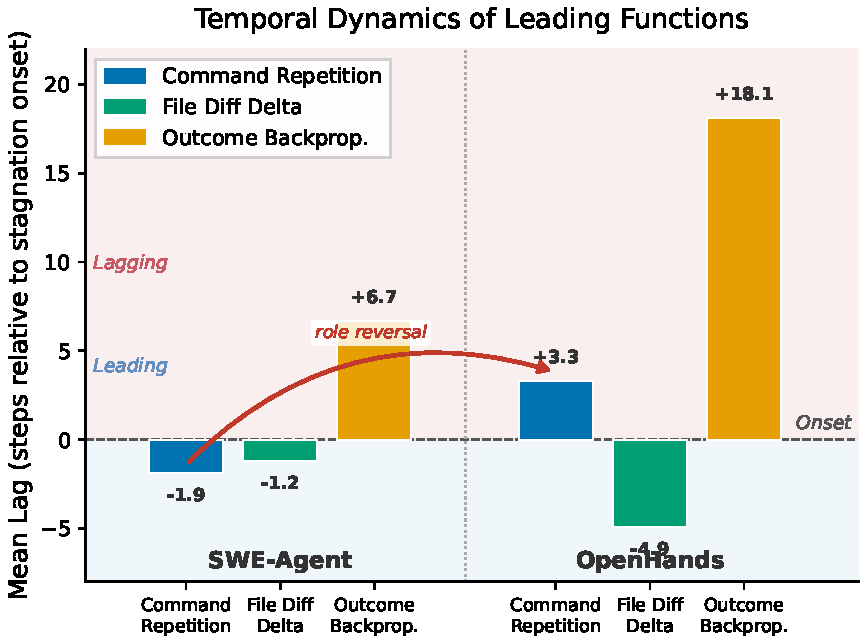
\includegraphics[width=\columnwidth]{../../figures/paper/fig_lf_temporal.pdf}
\caption{Temporal roles of labeling functions relative to stagnation onset on SWE-Agent. cmd\_rep leads ($-1.87$ steps), file\_diff is near-concurrent ($-1.20$), outcome\_bp lags ($+6.70$). Inset: OH reversal where cmd\_rep becomes lagging.}
\label{fig:lf_temporal}
\end{figure}

All pairwise differences are significant (Bonferroni-corrected: cmd\_rep vs.\ file\_diff $p{=}1.44{\times}10^{-26}$, cmd\_rep vs.\ outcome\_bp $p{=}6.67{\times}10^{-39}$, file\_diff vs.\ outcome\_bp $p{=}3.47{\times}10^{-47}$).

%-------------------------------------------------------------------
\subsection{Gold Set Validation Protocol}
\label{sec:app_gold_set}

We sample 650 windows stratified along two axes---\emph{confidence} (balanced across conf${=}1$, conf${=}2$, and conf${=}3$ strata) and \emph{trajectory position} (early, middle, and late thirds)---for non-circular evaluation.
Of these, 512 received at least one annotation.

Three CS graduate students independently label each window as stagnation or progress using an operational definition: \emph{a window is stagnation if the agent's actions within it do not make meaningful progress toward solving the task, regardless of whether the actions appear diverse or purposeful}.
Annotators receive the $k{=}5$ action descriptions with full command outputs and file diffs, but \emph{not} the task outcome (resolved/unresolved), preventing information leakage from $\lambda_3$.

\paragraph{Evaluation sets.}
We define three evaluation sets from the 512 annotated windows:
Set~A ($N{=}52$): windows labeled by all three annotators (used for IAA);
Set~B ($N{=}505$): windows where ${\geq}$2 annotators agree on the gold label (primary evaluation);
Set~C ($N{=}512$): all windows with ${\geq}$1 annotation.
Table~\ref{tab:gold_batch1} reports detection performance on Set~B.

\paragraph{Inter-annotator agreement.}
\label{sec:app_iaa}
On the 52 three-annotator windows (Set~A), Fleiss' $\kappa{=}0.39$ (fair agreement); pairwise Cohen's $\kappa$ ranges from 0.33 to 0.49.
The moderate agreement reflects the inherent subjectivity of stagnation boundaries: an agent exploring alternative strategies may appear stuck or productive depending on annotator interpretation, particularly when actions are semantically diverse but ultimately unproductive.
This subjectivity motivates the weak supervision approach: rather than relying on expensive and inherently noisy human labels, the system derives silver labels from complementary heuristic signals.

\paragraph{Gold detection results.}
Table~\ref{tab:gold_batch1} reports model performance against Set~B gold labels.

\begin{table}[h]
\centering
\small
\begin{tabular}{llcc}
\toprule
\textbf{Method} & \textbf{Scope} & $N$ & \textbf{Macro-F1} \\
\midrule
Structural GB   & SWE-only & ${\sim}$335 & \textbf{0.877} \\
TWV Probe       & SWE-only & ${\sim}$335 & 0.854 \\
\midrule
Structural GB   & All      & 505 & \textbf{0.839} \\
Structural RF   & All      & 505 & \underline{0.811} \\
MV Labels       & All      & 505 & 0.798 \\
GRU Probe       & SWE-only & ${\sim}$335 & 0.790 \\
\bottomrule
\end{tabular}
\caption{Gold set detection results (Set~B, $N{=}505$, ${\geq}$2-annotator agreement; 3 CS graduate students, Fleiss' $\kappa{=}0.39$). GB outperforms MV by 4.2\,pp (paired bootstrap $p{<}0.001$, $B{=}10{,}000$). Probe models are evaluated on the SWE-only subset ($N{\approx}335$) due to missing OH embeddings; scope-matched, GB (0.877) exceeds TWV Probe (0.854). \textbf{Bold} = best within scope, \underline{underline} = second.}
\label{tab:gold_batch1}
\end{table}

GB vs.\ MV: $+$4.2\,pp ($p{<}0.001$); GB vs.\ RF: $+$2.9\,pp ($p{<}0.001$); GB vs.\ GRU Probe: $+$5.0\,pp on the full set (paired bootstrap on shared SWE-only subset: $+$8.8\,pp, $p{<}0.001$).
On the SWE-only subset, GB (0.877) exceeds TWV Probe (0.854) by 2.3\,pp ($p{=}0.056$, not significant at $\alpha{=}0.05$); the TWV advantage in the overall ranking reflects scope mismatch, not superior detection.
Set~A ($N{=}52$) and Set~C ($N{=}512$) yield consistent rankings (GB $>$ MV in all sets).

%-------------------------------------------------------------------
\subsection{Feature Overlap Ablation Table}
\label{sec:app_feature_overlap}

\begin{table}[h]
\centering
\small
\begin{tabular}{lccc}
\toprule
\textbf{Feature Set} & \textbf{\#Feat} & \textbf{In-Dom.} & \textbf{Cross-Ag.} \\
\midrule
Full (all 30) & 30 & 0.9951 & 0.9674 \\
LF-overlap only & 11 & 0.9937 & \textbf{0.9770} \\
Residual only & 19 & 0.9515 & 0.5656 \\
\midrule
\multicolumn{4}{l}{\emph{Leave-one-group-out (cross-coding-agent)}} \\
$-$ cmd\_rep ($\lambda_1$) & 25 & --- & 0.5620 \\
$-$ file\_diff ($\lambda_2$) & 25 & --- & 0.6590 \\
$-$ outcome\_bp ($\lambda_3$) & 29 & --- & 0.9660 \\
\bottomrule
\end{tabular}
\caption{Feature overlap ablation (GB). In-Dom.\ = SWE-Agent in-domain macro-F1; Cross-Ag.\ = SWE-Agent $\to$ OpenHands zero-shot. Top: on all OH windows, LF-overlap features alone exceed the full model cross-coding-agent ($+$1.0\,pp; on conf${\geq}$2, direction reverses by $-$0.71\,pp); residual features collapse. Bottom: removing each LF-group individually; cmd\_rep features account for the largest transfer drop ($-$40.6\,pp).}
\label{tab:feature_overlap}
\end{table}

%-------------------------------------------------------------------
\subsection{Cycle Detector Baseline}
\label{sec:app_cycle_detector}

We evaluate n-gram cycle detectors as external baselines---methods that flag stagnation when an exact n-gram of consecutive commands recurs within a window.

\begin{table}[h]
\centering
\small
\begin{tabular}{lcccc}
\toprule
& \multicolumn{2}{c}{\textbf{SWE In-Domain}} & \multicolumn{2}{c}{\textbf{OH Cross-Agent}} \\
\cmidrule(lr){2-3} \cmidrule(lr){4-5}
\textbf{Method} & Silver & Gold & All & Oracle \\
\midrule
3-gram cycle & 0.721 & \textbf{0.841} & 0.530 & --- \\
2-gram cycle & 0.661 & 0.840 & 0.520 & --- \\
Oracle ceiling & --- & --- & --- & 0.552 \\
\midrule
Structural GB & \textbf{0.995} & 0.839 & \textbf{0.967} & --- \\
\bottomrule
\end{tabular}
\caption{Cycle detector vs.\ structural features. In-domain: SWE-Agent test set (silver = conf${\geq}$2 silver labels; gold = Set~B gold labels). Cross-agent: SWE-Agent $\to$ OpenHands zero-shot. Cycle detectors match structural GB on gold in-domain (${\sim}$0.84) but collapse on cross-agent transfer ($-$43.7\,pp gap), confirming that cross-agent generalization---not in-domain detection---is the genuine structural contribution.}
\label{tab:cycle_detector}
\end{table}

The silver--gold inversion for cycle detectors (silver 0.721 vs.\ gold 0.841) indicates that silver labels penalize cycle detectors for missing non-repetitive stagnation, while human annotators judge overt repetition as clear stagnation.
Structural features show the opposite pattern (silver 0.995 vs.\ gold 0.839): silver labels reward LF-reconstructibility, while gold labels impose a ceiling reflecting genuine detection difficulty.
The cross-agent collapse ($-$43.7\,pp) demonstrates that n-gram repetition is an agent-specific surface pattern: OpenHands stagnation rarely manifests as exact command repetition, requiring the richer feature vocabulary that structural classifiers provide.

%-------------------------------------------------------------------
\subsection{Encoder Cross-Agent Transfer}
\label{sec:app_encoder_cross}

\begin{table}[h]
\centering
\small
\begin{tabular}{lccc}
\toprule
\textbf{Encoder} & \textbf{SWE In-Dom.} & \textbf{OH Cross-Ag.} & \textbf{Gap to GB} \\
\midrule
E5-large-v2 & 0.941 & \textbf{0.733} & $-$25.9\,pp \\
BGE-M3 & \textbf{0.941} & 0.666 & $-$30.1\,pp \\
Qwen3-0.6B & 0.906 & 0.598 & $-$36.9\,pp \\
\bottomrule
\end{tabular}
\caption{Encoder cross-agent transfer (OH conf${\geq}$2). All probes use the same GRU architecture. In-domain performance is encoder-agnostic (0.91--0.94), but cross-agent transfer varies substantially (0.60--0.73, 13.5\,pp spread). Even the best probe (E5-large, 0.733) remains 25.9\,pp below structural GB (0.992 conf${\geq}$2).}
\label{tab:encoder_cross}
\end{table}

%-------------------------------------------------------------------
\subsection{Bidirectional Transfer}
\label{sec:app_reverse_transfer}

\begin{table}[h]
\centering
\small
\begin{tabular}{llcccc}
\toprule
& & \multicolumn{2}{c}{\textbf{Conf${\geq}$2}} & \multicolumn{2}{c}{\textbf{All Windows}} \\
\cmidrule(lr){3-4} \cmidrule(lr){5-6}
\textbf{Direction} & & GB & RF & GB & RF \\
\midrule
SWE$\to$OH & & 0.992 & \textbf{0.996} & \textbf{0.967} & 0.912 \\
OH$\to$SWE & & \textbf{0.995} & \textbf{0.995} & 0.937 & \textbf{0.953} \\
\bottomrule
\end{tabular}
\caption{Bidirectional cross-agent transfer (macro-F1). Conf${\geq}$2 performance is symmetric (${\leq}$0.3\,pp difference), confirming that structural stagnation patterns are agent-agnostic rather than training-source-dependent. On all windows, OH$\to$SWE transfer is slightly lower (GB $-$3.0\,pp, RF $+$4.1\,pp), reflecting distributional differences in conf${=}1$ labels.}
\label{tab:reverse_transfer}
\end{table}

%-------------------------------------------------------------------
\subsection{6-LF Label Model Analysis}
\label{sec:app_6lf}

To test whether the 3-LF label model failure (\S\ref{sec:temporal_label_models}) stems from insufficient LF quantity, we expand to 6 LFs by adding three additional functions (error repetition, output stagnation, and edit distance decay) and evaluate against gold labels.

\begin{table}[h]
\centering
\small
\begin{tabular}{lcc}
\toprule
\textbf{Method} & \textbf{6-LF Gold F1} & $\Delta$ \textbf{vs.\ 6-LF MV} \\
\midrule
6-LF MV & 0.719 & --- \\
TWV ($\sigma{=}5$) & 0.744 & $+$2.4\,pp \\
Lag-HMM & 0.764 & $+$4.5\,pp \\
HMM & \textbf{0.784} & $+$6.5\,pp \\
\bottomrule
\end{tabular}
\caption{6-LF label model evaluation against gold labels. HMM recovers $+$6.5\,pp over 6-LF MV, but the absolute score (0.784) remains below 3-LF MV (0.798). The gains reflect recovery from label quality degradation introduced by low-quality LFs, not improvement over simpler high-quality configurations.}
\label{tab:6lf_tlm}
\end{table}

The 6-LF regime increases inter-LF conflict to 42\%, enabling temporal models to add value: HMM gains $+$6.5\,pp over 6-LF MV, confirming that the 3-LF failure stems from insufficient conflict rather than model limitations.
However, the best 6-LF score (HMM 0.784) remains below 3-LF MV (0.798) in absolute terms---the additional LFs introduce noise that temporal aggregation partially but not fully recovers.
This suggests that TLM value lies in \emph{robustness to low-quality LFs} rather than outperforming simpler high-quality configurations.

%-------------------------------------------------------------------
\subsection{Third-Agent Transfer (ACR)}
\label{sec:app_acr}

We evaluate transfer to a third coding agent (ACR) to test generalization beyond the SWE-Agent / OpenHands pair.

\paragraph{Original 3-LF pipeline.}
Direct transfer produces GB 0.608 macro-F1 on ACR, with the conf${\geq}$2 subset degenerating to only 5 samples---insufficient for meaningful evaluation.
The collapse is driven by LF coverage: $\lambda_1$ (command repetition) and $\lambda_3$ (outcome backpropagation) fire on $<$3\% of ACR windows.

\paragraph{Adapted LF pipeline.}
Adapting LFs to ACR-specific patterns (4 adapted LFs replacing the original 3) yields mixed results: RF improves by $+$10.4\,pp (0.665$\to$0.769) while GB drops by $-$3.6\,pp.
Two of the four adapted LFs (output\_stagnation, error\_repetition) achieve zero coverage on ACR, indicating that agent-specific LF design remains necessary.
LF portability---not model architecture---is the bottleneck for third-agent transfer.

%-------------------------------------------------------------------
\subsection{Non-SE Domain Pilot}
\label{sec:app_nonse}

To probe domain transferability beyond software engineering, we evaluate the structural feature pipeline on ALFWorld \citep{yao2023react}, a household robot task environment.

Of the 30 structural features, 23 transfer directly (trajectory statistics, text statistics, repetition ratios); 7 require domain adaptation (file operation counts, edit-specific features).
The three LFs achieve 53--100\% coverage on ALFWorld trajectories: command repetition ($\lambda_1$) and output patterns transfer naturally, while file diff ($\lambda_2$) requires reinterpretation as ``state change detection.''
These results suggest the structural monitoring approach generalizes beyond software engineering, though full evaluation requires domain-specific gold labels.

%-------------------------------------------------------------------
\subsection{SHAP Feature Importance}
\label{sec:app_shap}

\begin{figure}[h]
\centering
\includegraphics[width=\columnwidth]{../../figures/d073/shap_feature_importance.pdf}
\caption{SHAP feature importance for the structural GB classifier (SWE-Agent in-domain). Repetition-based features (unique\_cmd\_ratio, max\_repeat\_ratio) dominate, consistent with $\lambda_1$'s role as the primary stagnation signal. File operation features contribute moderately, while text statistics have minimal impact.}
\label{fig:shap}
\end{figure}

%-------------------------------------------------------------------
\subsection{Trajectory Visualization}
\label{sec:app_trajectory}

\begin{figure}[h]
\centering
\includegraphics[width=\columnwidth]{../../figures/d073/trajectory_visualization.pdf}
\caption{Example agent trajectory with stagnation labels. Colored regions indicate silver-labeled stagnation (red) and progress (green) windows. The trajectory illustrates semantic stagnation: the agent issues diverse commands but makes no effective progress, with stagnation onset detected before overt repetition begins.}
\label{fig:trajectory}
\end{figure}

%-------------------------------------------------------------------
\subsection{Calibration Analysis}
\label{sec:app_calibration}

\begin{figure}[h]
\centering
\includegraphics[width=\columnwidth]{../../figures/d073/reliability_diagrams.pdf}
\caption{Reliability diagrams for the structural GB and GRU probe classifiers. GB is well-calibrated across all confidence bins; the probe shows slight overconfidence at high predicted stagnation probability.}
\label{fig:reliability}
\end{figure}

%-------------------------------------------------------------------
\subsection{Early Termination Analysis}
\label{sec:app_pareto}

\begin{figure}[h]
\centering
\includegraphics[width=\columnwidth]{../../figures/pareto_curve.pdf}
\caption{Pareto frontier of task resolution rate vs.\ compute savings under early termination triggered by stagnation detection. Structural GB achieves the best trade-off, enabling 15--30\% compute reduction with $<$2\% resolution rate loss. The probe achieves comparable savings only after fine-tuning on target-agent data.}
\label{fig:pareto}
\end{figure}
